\documentclass[border=6pt]{standalone}
\usepackage{tikz}
\usetikzlibrary{arrows.meta,positioning,calc,decorations.pathreplacing}
\begin{document}
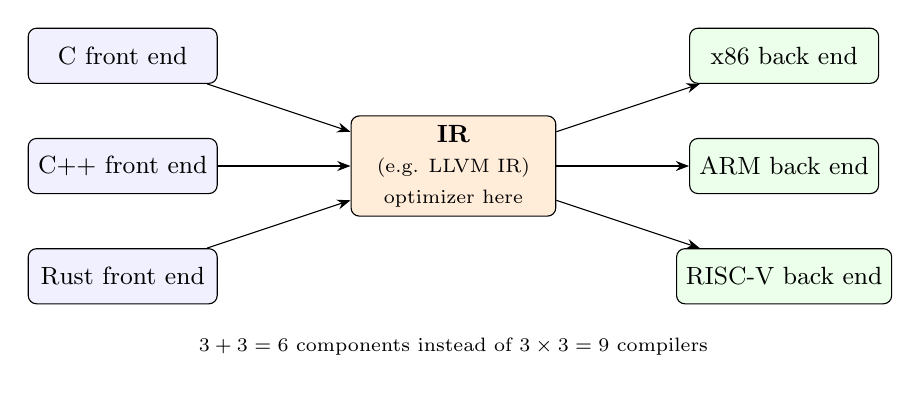
\begin{tikzpicture}[>=Stealth,font=\small,
 fe/.style={draw,rounded corners=3pt,fill=blue!6,minimum width=2.4cm,minimum height=0.7cm},
 be/.style={draw,rounded corners=3pt,fill=green!8,minimum width=2.4cm,minimum height=0.7cm}]
\node[fe] (c) at (0,1.4) {C front end};
\node[fe] (cpp) at (0,0) {C++ front end};
\node[fe] (r) at (0,-1.4) {Rust front end};
\node[draw,rounded corners=3pt,fill=orange!15,minimum width=2.6cm,minimum height=1.2cm,align=center] (ir) at (4.2,0) {\textbf{IR}\\{\scriptsize (e.g. LLVM IR)}\\{\scriptsize optimizer here}};
\node[be] (x) at (8.4,1.4) {x86 back end};
\node[be] (a) at (8.4,0) {ARM back end};
\node[be] (v) at (8.4,-1.4) {RISC-V back end};
\foreach \s in {c,cpp,r} \draw[->] (\s) -- (ir);
\foreach \t in {x,a,v} \draw[->] (ir) -- (\t);
\node[font=\scriptsize,align=center] at (4.2,-2.3) {$3 + 3 = 6$ components instead of $3 \times 3 = 9$ compilers};
\end{tikzpicture}
\end{document}
